\documentclass{article}
\usepackage[utf8]{inputenc}
\usepackage{graphicx}
\graphicspath{ {images/} }
\title{CS763 poisoning data}
\author{pierre.petrella }
\date{September 2019}

\begin{document}
\maketitle
\tableofcontents
\newpage
\section*{How secure are our classifiers? }
% ----------------- subsection---------------------
\subsection {potential threats of ML pipeline poisoning}
\paragraph{}
Machine learning systems have made itself necessary in this new data era requiring data analysis that can only be managed by automated processes. It is more precisely used for image recognition from distinguishing cats from dogs, red lights from green lights to facial recognition. 
\paragraph{}
Unfortunately these machine learning systems can be compromised. They are now becoming the weakest part of the security chain and consequently of the whole system. If no precautions are taken, this weakness can be used as a weapon by the attackers.

% ----------------- subsection---------------------
\subsection{General attack on a ML Pipeline}
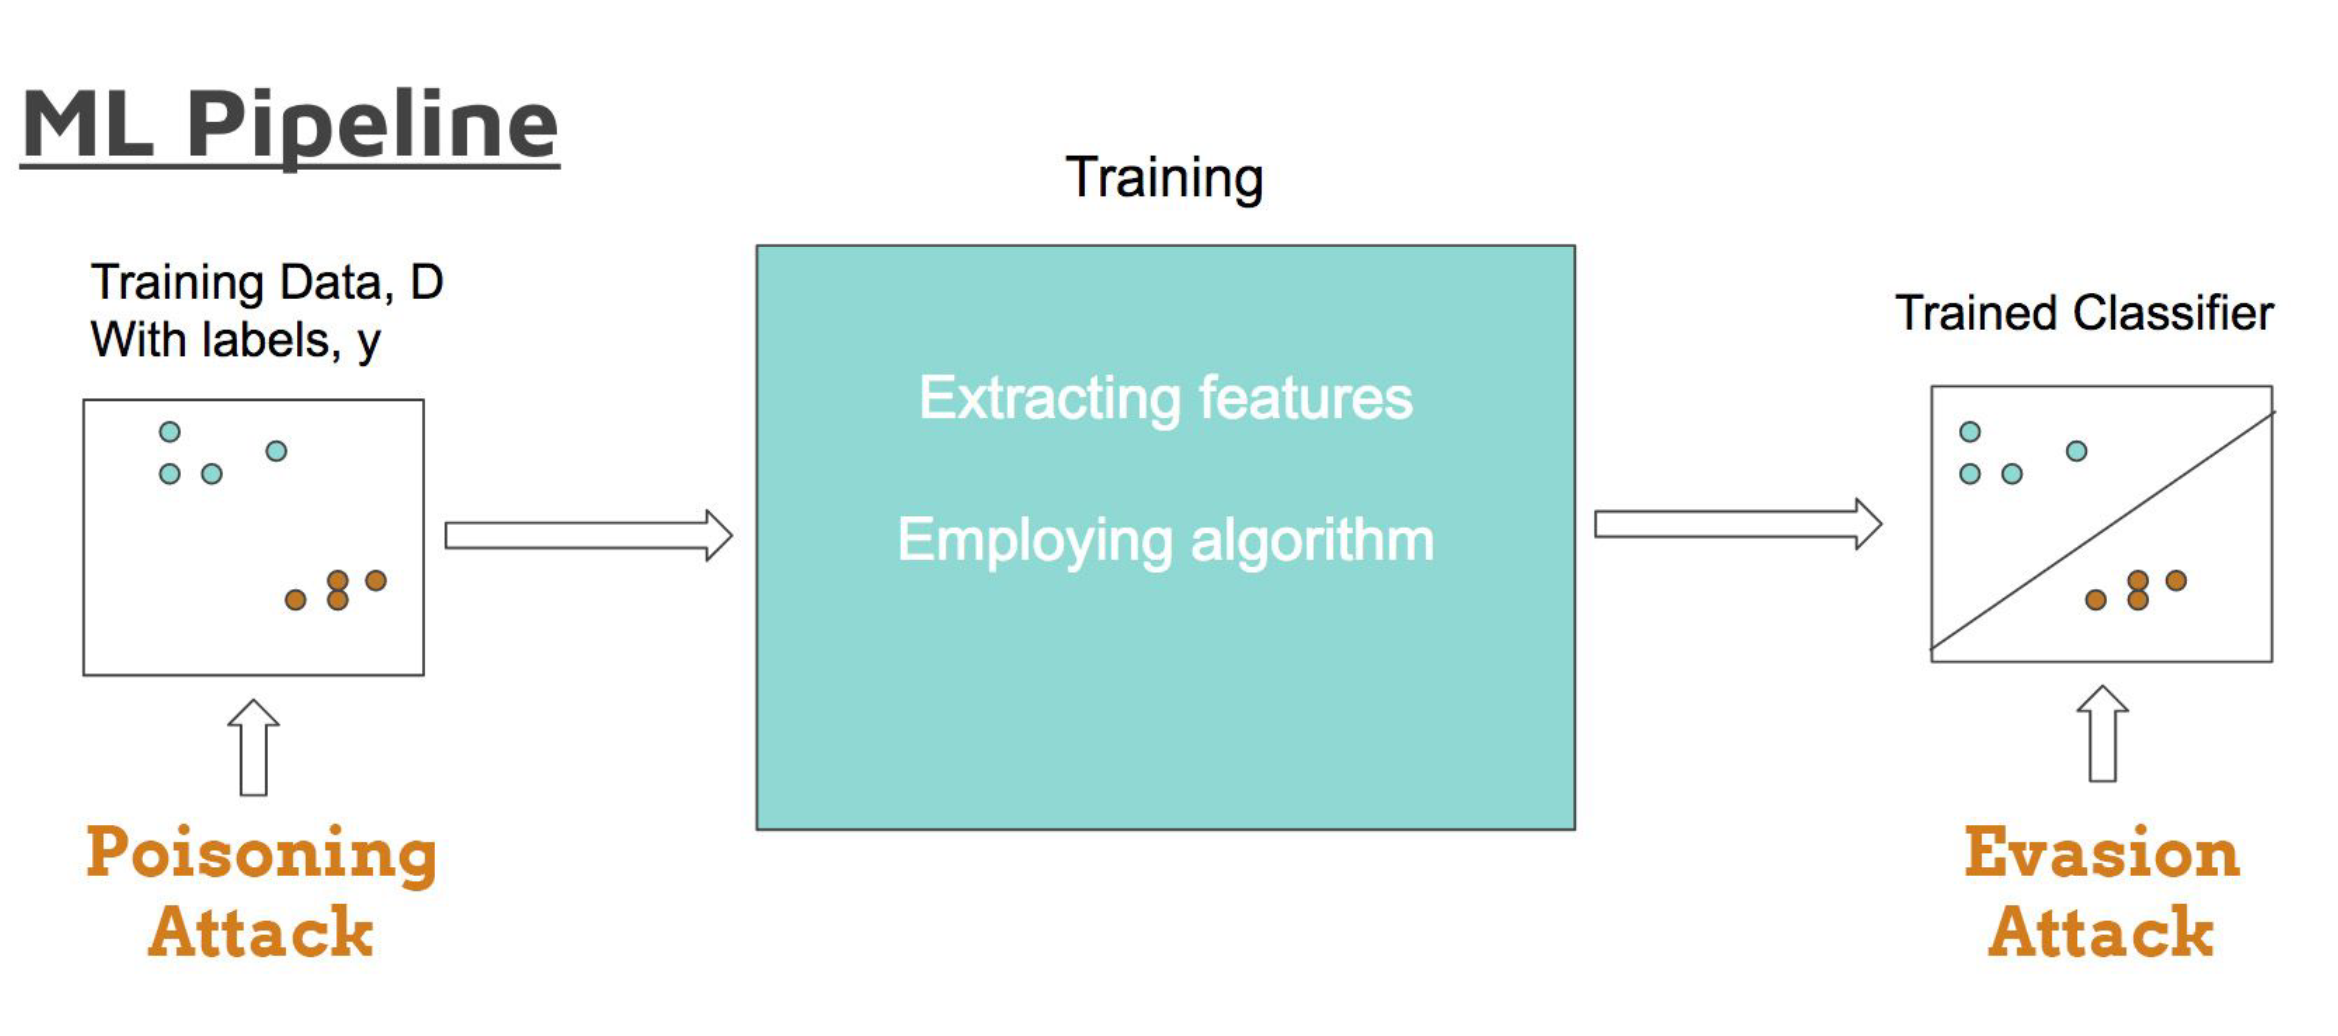
\includegraphics[scale=0.3]{MLpipeline.png}
% ----------------- section------------------------
\section{Targeted clean labor poisoning attacks on Neutral Networks}

% ----------------- subsection---------------------
\subsection{Assumptions}

The attacker has:
\begin{enumerate}
  \item No knowledge of the training data
  \item No control over the target instance during test time
  \item No control over labelling of data for training
  \item Knowledge of the model and it's parameters
\end{enumerate}
\paragraph{}
These restriction are quite strict on the attacker. This implies that the data poisoning requires minimal intrusion which makes it difficult to detect for the ML model.
% ----------------- subsection---------------------
\subsection{Properties}

\subsubsection*{Clean labels}
\paragraph{}
There are various types of poisoning attacks. In this paper, we are focusing on clean labels opposed to poisoning that involve tampering with the labels. clean labels allows to poison a training set with minimal intrusion as the poisoned image can simply be uploaded online and wait to be used by a ML model.

\subsubsection*{Targeted}
\paragraph{}
This type of attack is built to affect one image specifically and not tamper with the other ones. This allows the poisoning to happen without the Users noticing that the model was tampered with. the Degradation of the model should be unnoticeable.
\subsubsection*{good success rate}
\paragraph{}
If the poisoning is affecting the last more specific nodes of the ML model, we can assume that the poisoning will have a success rate of 100\% most of the time. 


% ----------------- subsection---------------------
\subsection{poisoning Attacks example}

\paragraph
We will be considering the Classifier that sorts between fish and dogs. The goal of the attacker will be to chose a specific picture of a fish and trick the ML model to think it is a dog. To do so he and insert a poisoned instance for fish class from dog a base instance. This poisoned picture which looks like a dog will be labeled accordingly and therefore trick the ML model.
\paragraph{}
Here are examples of poisoned dog images associated with the fish images they are targeting. We can see that the difference between the original and poisoned dog is indistinguishable to the human eye.   

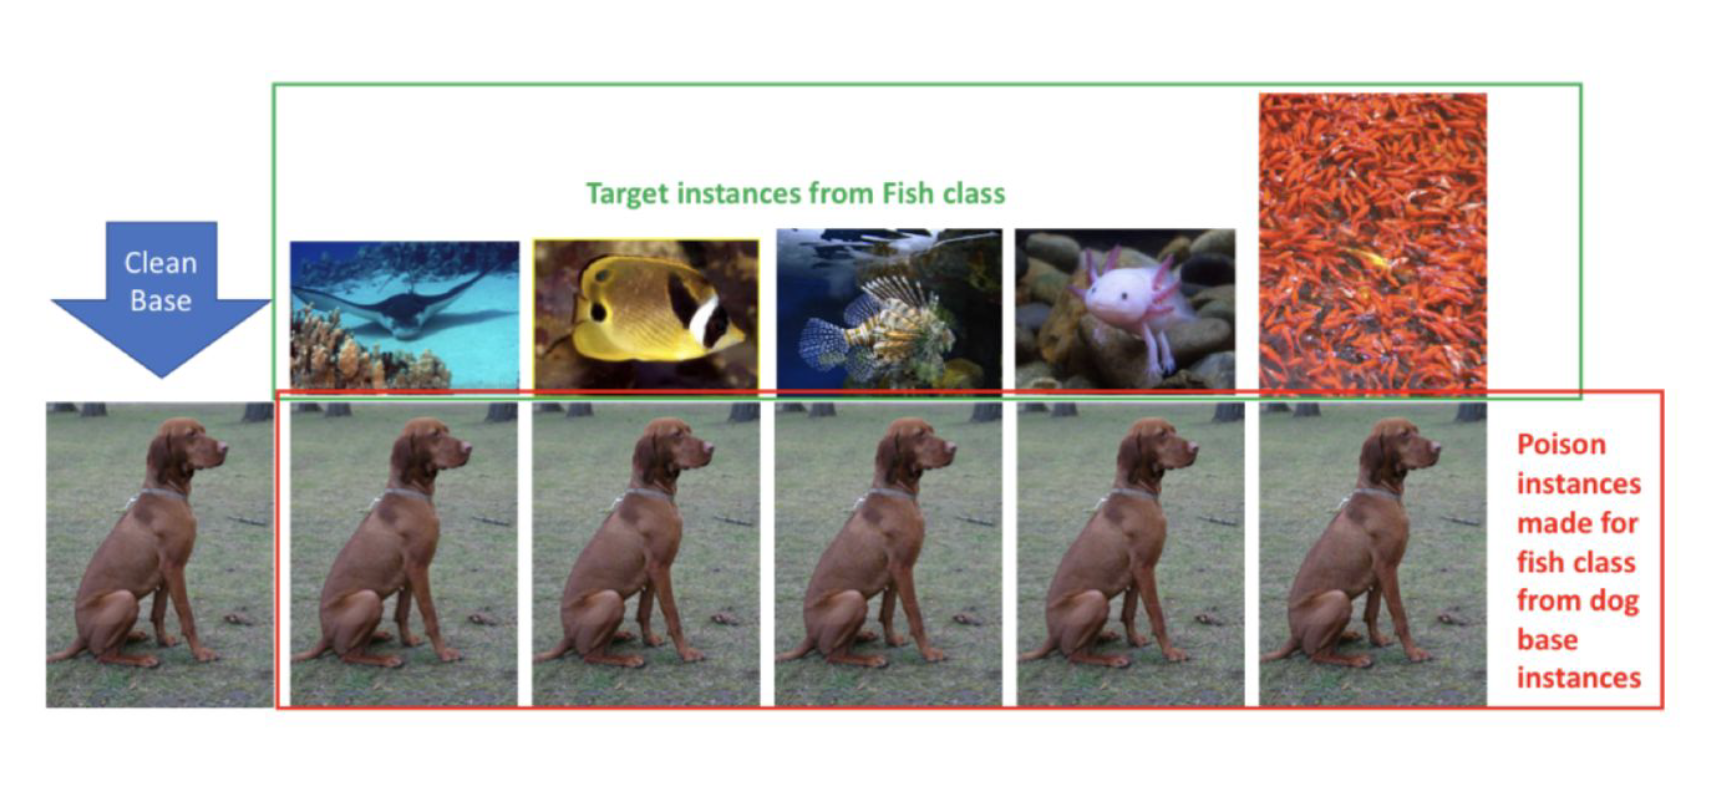
\includegraphics[scale=0.4]{ExamplePoisoning2.png}

% ----------------- subsection---------------------
\subsection{Transfer learning}
\paragraph{}
On way to train a new ML model is to use an existing working model that has been trained on a significantly big data set (Model A) and get rid of the last couple of layers. We then reconstruct the last layers using a relatively small data set to fine tune the model to distinguish cats and dogs for instance (Model B). 
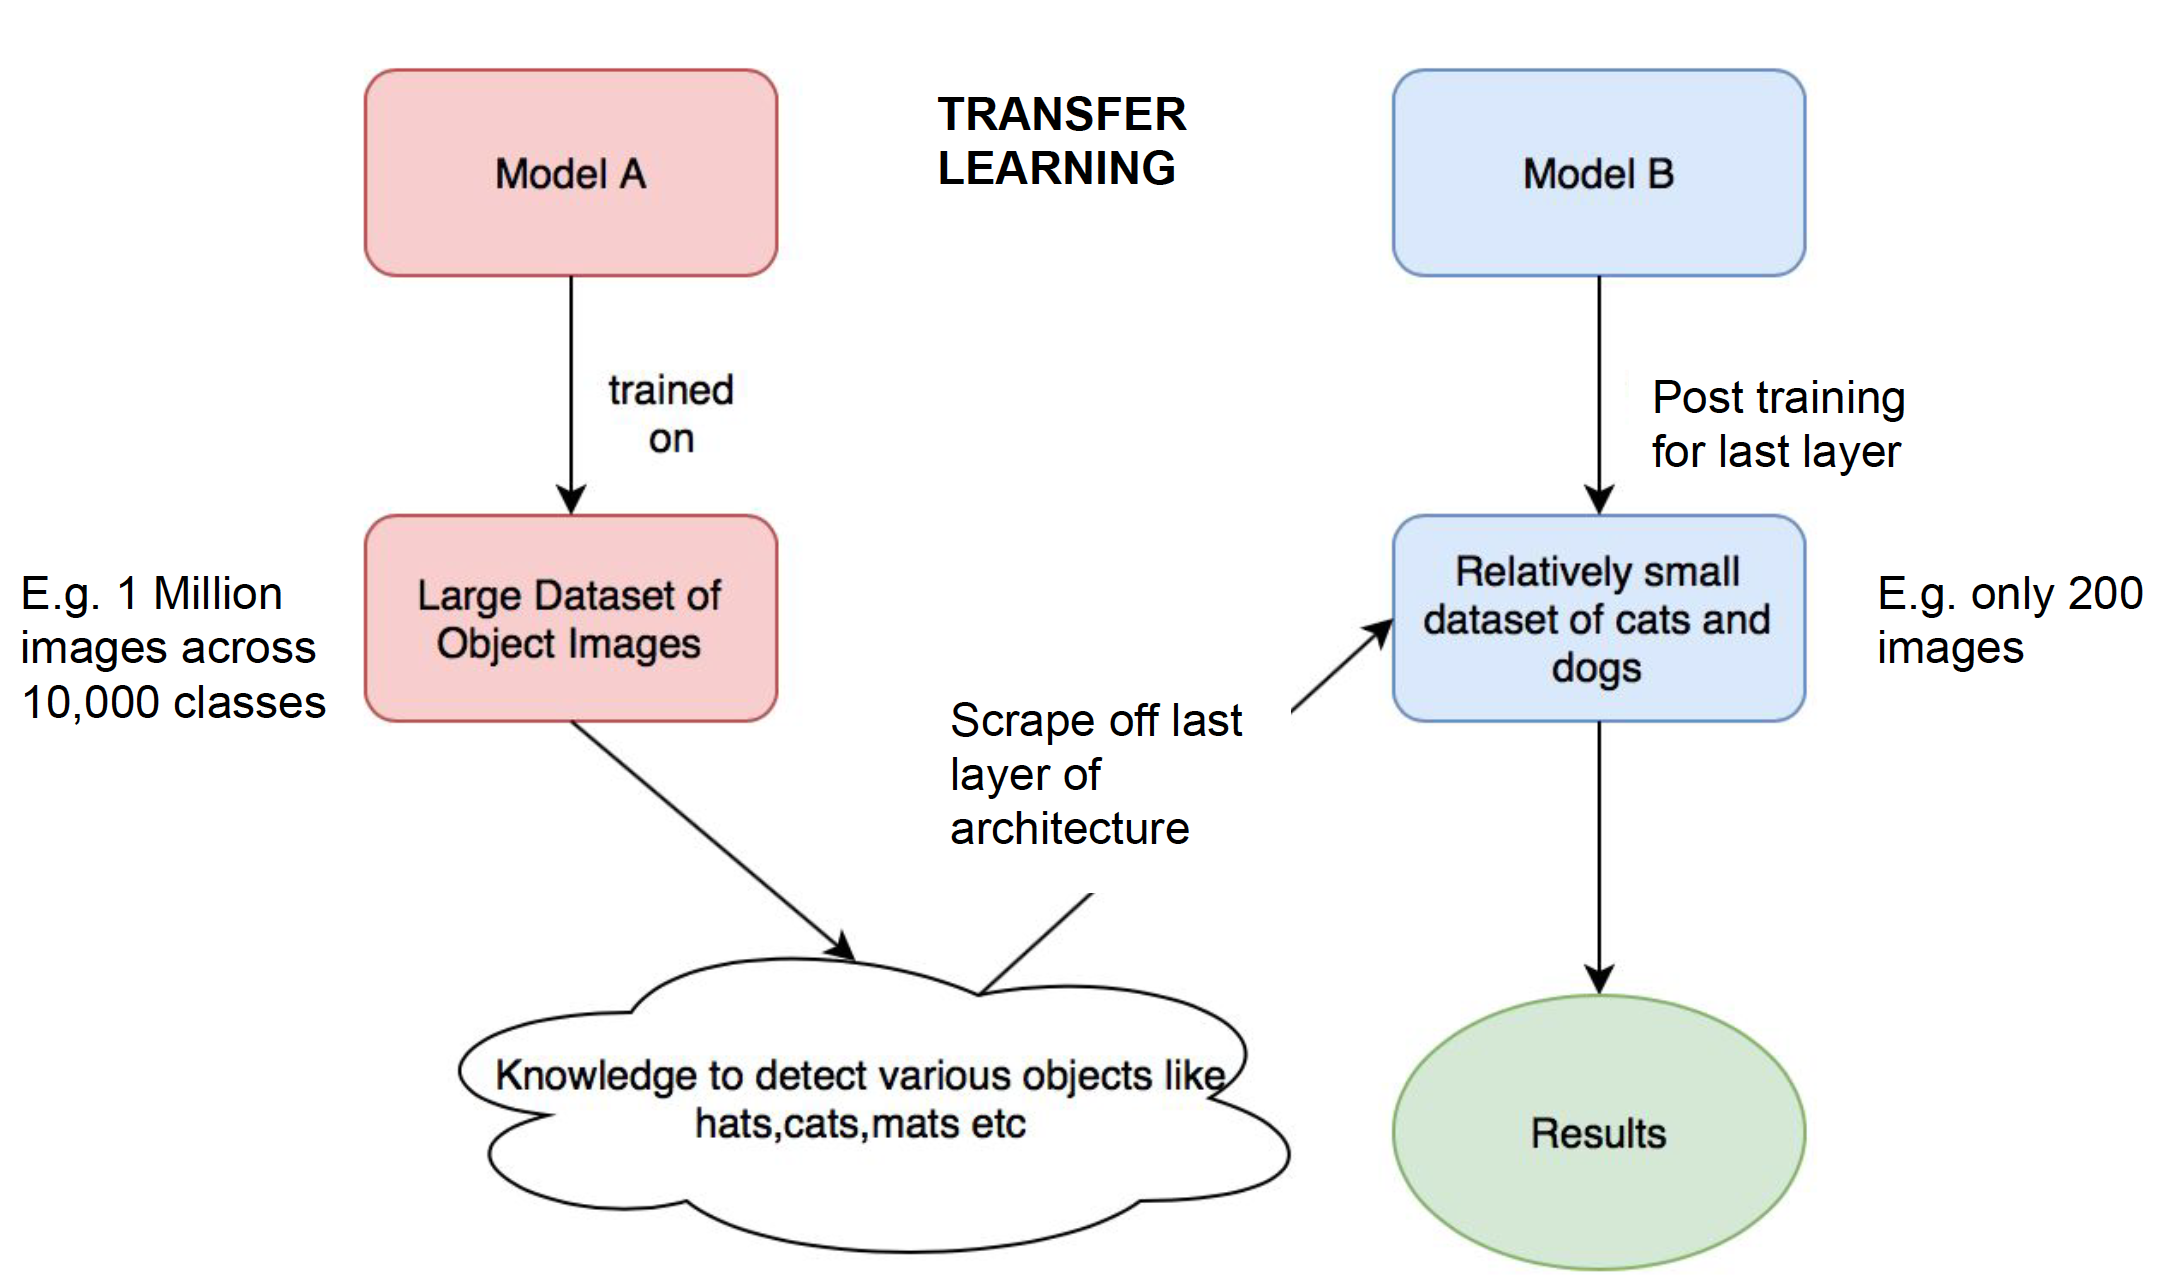
\includegraphics[scale=0.3]{MLTransfer.png}
\paragraph{}
These last layers are very susceptible to change making it an idea target for data poisoning. Transfer learning is an effective way to train a new model without requiring all the resources necessary to train a ML model from scratch. Unfortunately if the data set used to train the last layer has been tampered with classification accuracy can be easily tampered with. Here is another representation of Transfer learning. \\
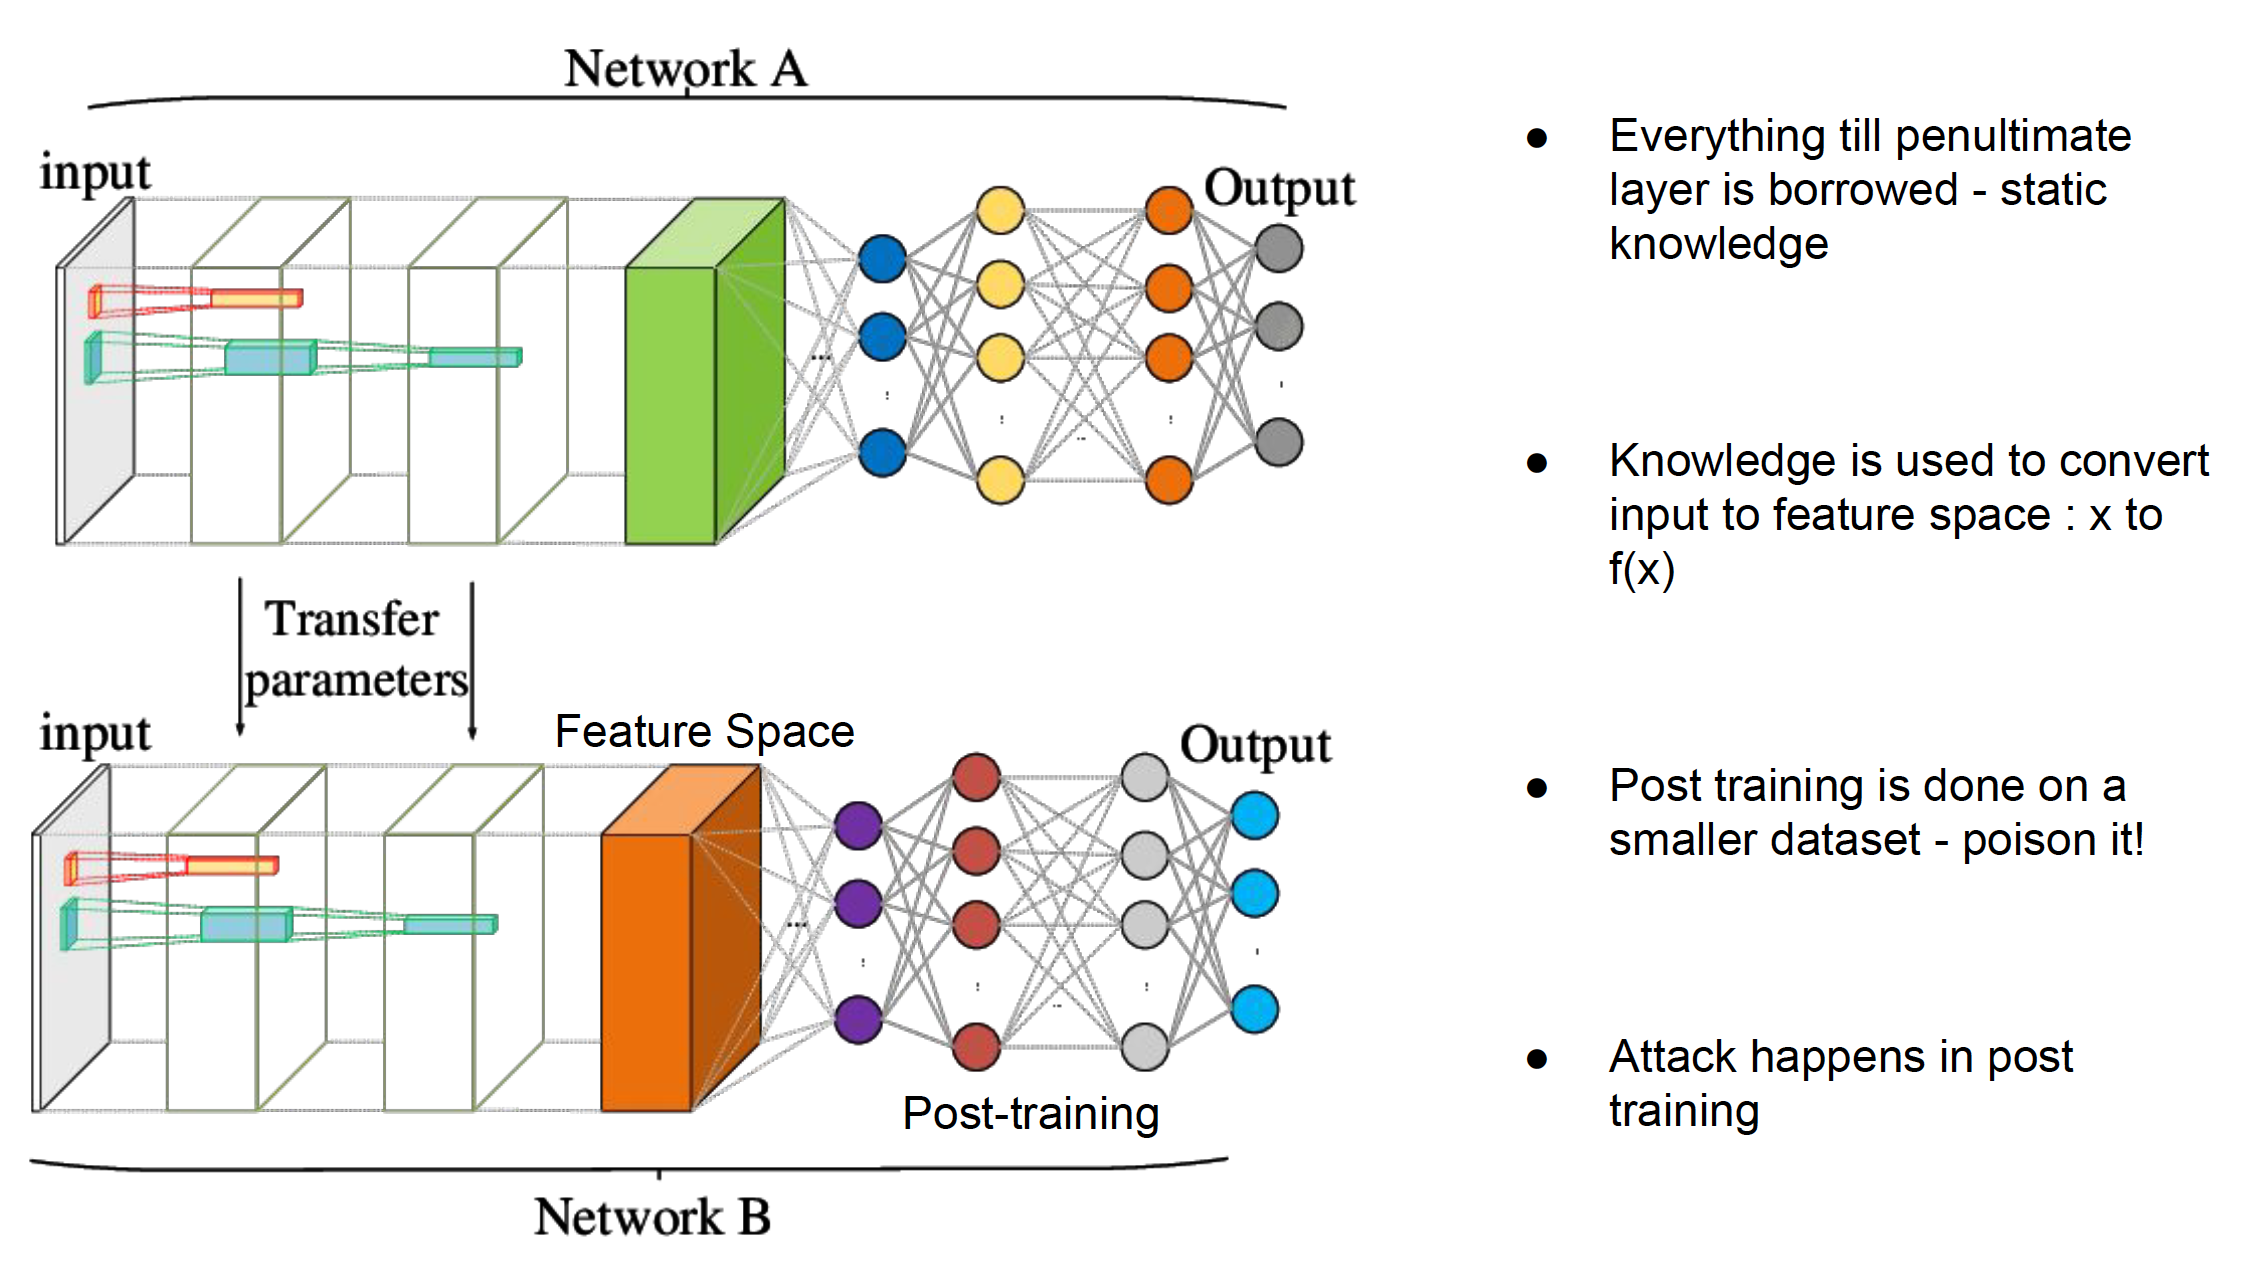
\includegraphics[scale=0.3]{MLTransfer2.png}

% ----------------- subsection---------------------
\subsection{Finding the poisoning}
\paragraph{}
The poisoning image must look like a dog but must have all the qualities of it's target (the fish). This will move the decision boundary from the initial doted line to the full line (see diagram). Now any pictures close enough to the targets characteristics will be on the "dog" side of the decision line and therefore be seen as a dog instead of a fish.

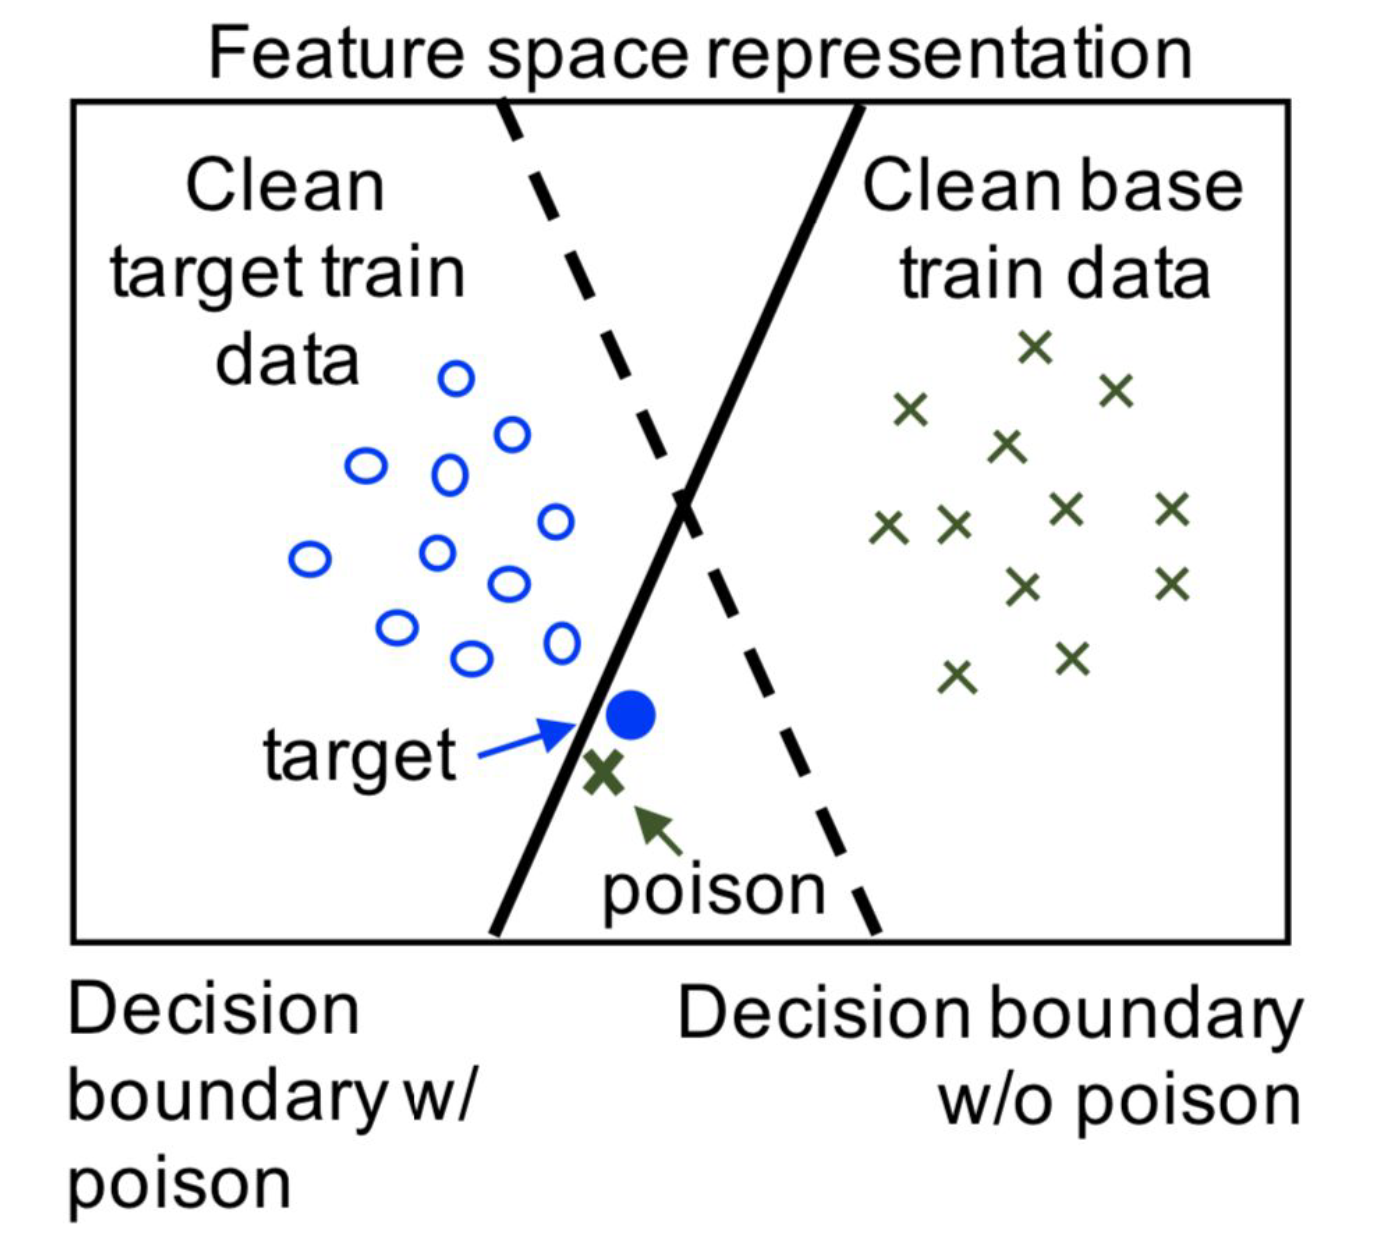
\includegraphics[scale=0.3]{DataLinePoison.png}
\paragraph{}
In order to create such a poisonous image we must find an image to satisfy this equation with X the image we want to find, t the target, b the initial "dog" image that we will modify and beta the importance we give to the similarity between the original a poisonous image: \\
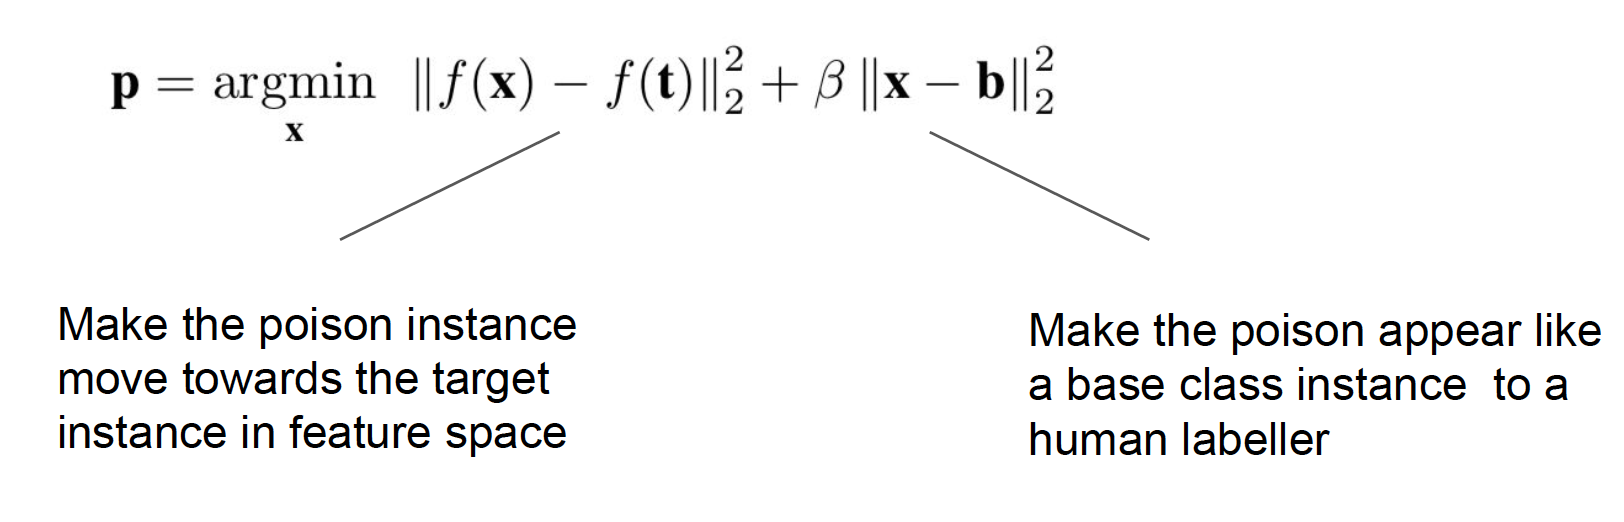
\includegraphics[scale=0.3]{Formula.png}

% ----------------- subsection---------------------
\subsection{Approach}
The protocol to follow to poison the data set is the following:

\begin{enumerate}
  \item Choose a target instance to misclassify
  \item Choose a base instance \& make imperceptible changes to it to get a poison
  \item Poison is created though an optimization based equation
  \item Inject poison into training data and let model be trained on poisoned dataset
\end{enumerate}

% ----------------- subsection---------------------
\subsection{Algorithm}
The algorithm to find the image consists of a forward backward iterative splitting procedure to find poison Iteratively. This is achieved by iterating these 2 steps:



\begin{enumerate}
  \item minimize distance to the target instance in feature space
  \item minimize distance from the base instance  in input space
\end{enumerate}

% ----------------- section------------------------
\section{Poisoning attacks in SVM (your part) }
\section*{Conclusion}
\end{document}
